\chapter{Asociación Calificada}
\begin{figure}[h]
\vspace{-.5cm}
	\centering
	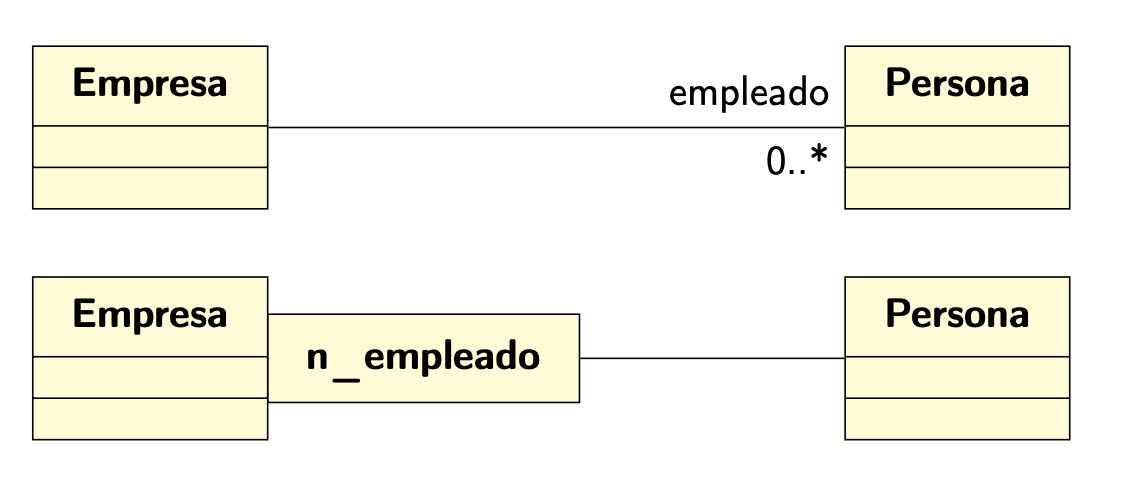
\includegraphics[width=\textwidth]{Imagenes/asc.png}
	\caption{Relaciones calificadas}
\end{figure}
Mediante esto, reducimos la multiplicidad en el lado muchos, haciendo las búsquedas mucho más eficientes.
Solamente podemos hacer uso de un atributo que sea \textit{clave primaria} de la clase.
Pasamos de 1 - muchos a 1 - 1.

Lo implementamos mediante un diccionario en la clase empresa.
Si la multiplicidad no se reduce, significa que dicho calificador no es \textbf{clave primaria} y por tanto, se pueden obtener diferentes valores para dicha clave.
\subsection{Implementación de la relacion}
\begin{center}
	\begin{lstlisting}[frame=single]
class Empresa{
 public:
//mediante un calificador, 
//encontramos un objeto de la clase Persona
   typedef std::map<T,Persona*>Bcalificada; 
//metodos de la clase
   void asocia(Persona&);
   const Bcalificada& getA()const;
 private:
   Bcalificada bc_;
};
class Persona{
 public:
//metodos propios de la clase
   typedef std::set<Empresa*>As;
   void asocia(Empresa&);
   const As& getB()const;
 private:
   T calificador; //calificador de tipo T(cualquier tipo de dato)
   As as_;
};
\end{lstlisting}
\end{center}